\documentclass[../diploma.tex]{subfiles}
 
\begin{document}

\begin{figure}[h!]
  \centering
  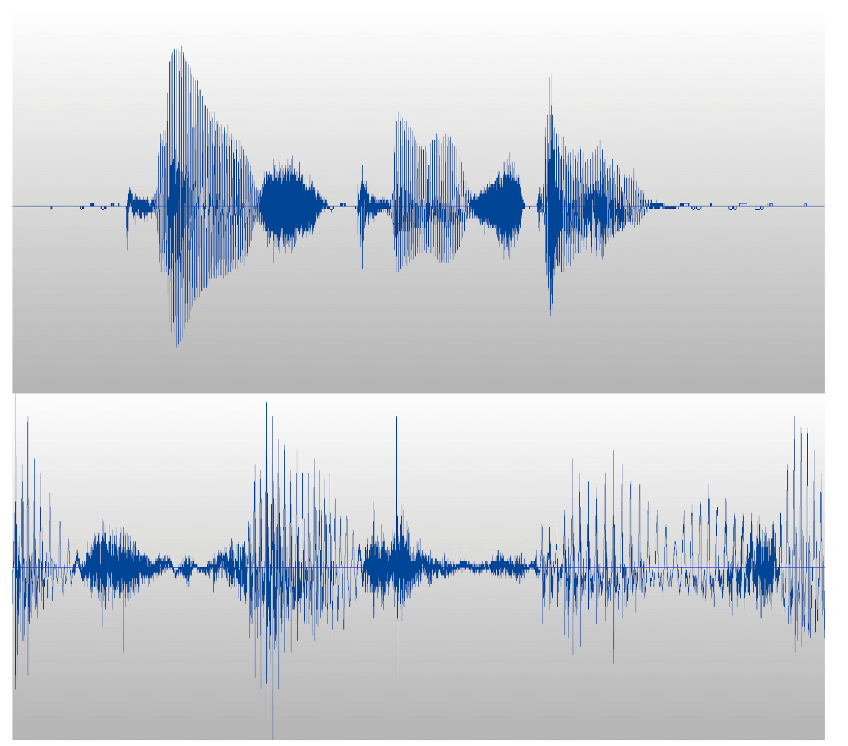
\includegraphics[scale=0.4]{img/compare}
  \caption{Сравнение сгенерированного сигнала с сигналом из обучающей выборки}
  \label{fig:perf}
\end{figure} 

Мы провели апробацию нашей модели в разных конфигурациях, с выбором признаков и подмножеств данных. Результаты можно увидеть в таблице \ref{table:experiments}

\begin{table}[]
\centering
\caption{Результаты экспериментов}
\label{table:experiments}
\begin{tabular}{|c|c|c|}
\hline
\textbf{Конфигурация WaveNet}                                                                                & \textbf{Данные}           & \textbf{Результат}                                                           \\ \hline
Без модификаций                                                                                              & весть корпус              & речеподобный звук                                                            \\ \hline
Без модификаций                                                                                              & одна фраза, много голосов & высокий гул                                                                  \\ \hline
Без модификаций                                                                                              & один голос, много фраз    & шум                                                                          \\ \hline
\begin{tabular}[c]{@{}c@{}}Глобальное условие:\\ ID говорящего\end{tabular}                                  & весь корпус              & речеподобный звук                                                            \\ \hline
\begin{tabular}[c]{@{}c@{}}Глобальное условие:\\ ID говорящего\end{tabular}                                  & одна фраза                & шум                                                                          \\ \hline
\begin{tabular}[c]{@{}c@{}}Глобальное условие:\\ пол говорящего\end{tabular}                                 & два голоса, много фраз    & шум                                                                          \\ \hline
\begin{tabular}[c]{@{}c@{}}Глобальное условие:\\ пол говорящего\end{tabular}                                 & два голоса, одна фраза    & шум                                                                          \\ \hline
\begin{tabular}[c]{@{}c@{}}Локальное условие:\\ текст\end{tabular}                                           & весь корпус               & шум                                                                          \\ \hline
Локальное условие:текст                                                                                      & одна фраза                & шум                                                                          \\ \hline
\begin{tabular}[c]{@{}c@{}}Локальное условие: \\ yandex-speech\end{tabular}                                  & весь корпус               & \begin{tabular}[c]{@{}c@{}}речеподобный звук\\ лучшего качества\end{tabular} \\ \hline
\begin{tabular}[c]{@{}c@{}}Локальное условие: \\ yandex-speech\end{tabular}                                  & одна фраза                & высокий гул                                                                  \\ \hline
\begin{tabular}[c]{@{}c@{}}Глобальное условие ID говорящего\\ + локальное условие yandex-speech\end{tabular} & весь корпус               & шум                                                                          \\ \hline
\begin{tabular}[c]{@{}c@{}}Глобальное условие ID говорящего\\ + локальное условие yandex-speech\end{tabular} & одна фраза                & шум                                                                          \\ \hline
\end{tabular}
\end{table}

Результаты генерации сложно описать в терминах численных характеристик, так как основным критерием качества мы считает естественность сгенерированного голоса.
В этом мы солидарны с авторами WaveNet, которые оценивали качество своих результатов с помощью некоторого Mean Optimal Score, который по сути основывался на оценках слушателей по пятибальной шкале (1: Плохо, 2: Слабо, 3: Удовлетворительно, 4: Хорошо, 5: Отлично). К сожалению, мы не можем совсем честно поставить эксперимент и получить оценку независимых слушателей, поэтому придётся поверить оценке автора диссертации.

\subsection{Сравнение качества результатов}
Для оценки качества независимым испытуемым проигрывались пары двухсекундных сгенерированных промежутков в двух разных конфигурациях и слушатель должен был сделать выбор, какая запись кажется ему более натуральной либо же заявить, что варианты для него индифферентны.
Для сравнения мы использовали конфигурации, показавшие лучшее качество генерируемого звука.
Результаты представлены в таблице \ref{table:natualness}.

% \caption{Сравнение натуральности генерируемых голосов}
% \label{table:natualness}

\begin{table}[]
\centering
\caption{Сравнение натуральности генерируемых голосов}
\label{table:natualness}
\begin{tabular}{|c|c|c|c|}
\hline
\multicolumn{4}{|c|}{Субъективное предпочтение(\%) в натуральности голоса}                                                                                                                                                                                                                                                                   \\ \hline
\begin{tabular}[c]{@{}c@{}}Без модификаций\\ на всём корпусе\end{tabular} & \begin{tabular}[c]{@{}c@{}}С глобальным условием\\ ID говорящего\\  на всём корпусе\end{tabular} & \begin{tabular}[c]{@{}c@{}}С локальным условием\\ yandex-speech на\\  всём корпусе\end{tabular} & \begin{tabular}[c]{@{}c@{}}Нет\\  предпочтения\end{tabular} \\ \hline
27                                                                        &                                                                                                  & \textbf{61}                                                                                     & 11                                                          \\ \hline
\textbf{34}                                                               & \textbf{34}                                                                                      &                                                                                                 & 31                                                          \\ \hline
                                                                          & 29                                                                                               & \textbf{56}                                                                                     & 15                                                          \\ \hline
\end{tabular}
\end{table}


\subsection{Производительность}

Мы считали на GPU Tesla K80 c 11 гигабайтами видеопамяти с поправками на виртуализацию.

Чтобы добиться значений функции потерь хотя бы как на рисунке \label{fig:perf} нам требуется около 4 суток. Генерация пяти секунд аудио занимает около часа.

\begin{figure}[h!]
  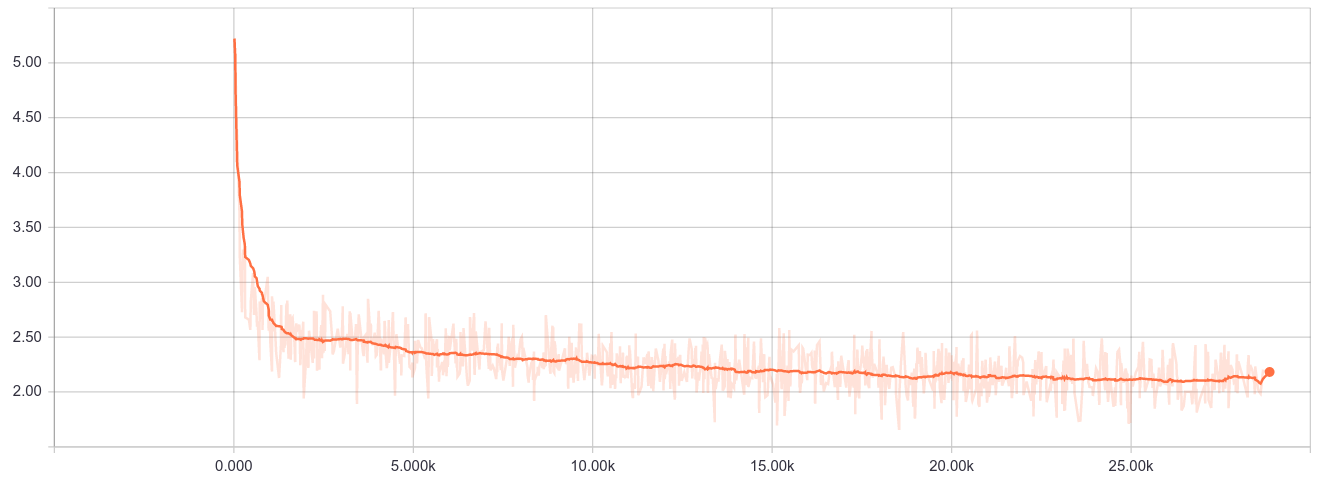
\includegraphics[scale=0.36]{img/perf}
  \caption{Изменение функции потерь в процессе обучения}
  \label{fig:perf}
\end{figure}

\subsection{Анализ экспериментов}

Исходы экспериментов можно просуммировать следующим образом:

\begin{enumerate}[resume]
    \item WaveNet реализован корректно.
\end{enumerate}

Это видно из экспериментов на модели без модификаций. Также показываем, что описательной силы архитектуры на сырых данных хватает, чтобы описать распределение порождаемое звуковым сигналом.

\begin{enumerate}[resume]
    \item Глобальные условия снижают качество.
\end{enumerate}

Почти во всех экспериментах с глобальными условиями не получилось хороших результатов.

\begin{enumerate}[resume]
    \item Использование результатов генерации независимой системы оправдывает себя  в качестве локального условия.
\end{enumerate}

Модель с этими настройками даёт лучшие показатели натуральности голоса, из тех, что нам удалось добиться. Однако хотелось бы добавить больше признаков, поскольку генерируемой речи не хватает структуры.

\begin{enumerate}[resume]
    \item Недостаточно качественных текстовых признаков.
\end{enumerate}

Тесты показали, что используемые нами текстовые признаки сказываются на качестве генерации отрицательно. Нам кажется, что основная проблема заключается в неточностях выравнивания и такие данные только запутывают модель. Возникла гипотеза, что с этой проблемой может помочь справиться реализация механизма внимания.

\begin{enumerate}[resume]
    \item Модель требует больше времени чтобы сойтись.
\end{enumerate}
Возможно, требуется больше времени для обучения сети, потому что как мы видим на рисунке \label{fig:perf} функция потерь не перестаёт падать, просто мы не можем себе позволить ждать так долго.
Однако такая гипотеза вызывает сомнения, потому что переобученные модели давали на выходе очень высокий неестественный звук.

\newpage
\end{document}

